 \documentclass [journal]{IEEEtran}

 \usepackage [pdftex]{graphicx}


% correct bad hyphenation here
 \hyphenation{op-tical net-works semi-conduc-tor}


 \begin{document}

 \title{Shared Ecosystem: Connecting IoT Devices Using Independent Search Engines And Neural Networks}

 \author{Eike Schultz, Universität zu Lübeck}

% The paper headers
 \markboth{Ambient Computing Seminar, June 2021}%
{Ambient Computing Seminar, June 2021}

% make the title area
 \maketitle

% As a general rule, do not put math, special symbols or citations
% in the abstract or keywords.
 \begin{abstract}
In recent years, the prevalence of Internet of Things devices has increased dramatically. More and more sensors reside in our environment, and most of them are not utilized to their full potential. To change that, W. G. Hatcher et al. have proposed a search engine to access these devices and the resources they provide. The use of accurate data in real-time increases the efficiency of many processes, from smart industry to individual transportation. This does pose a number of challenges needed to be overcome before such a search engine can be implemented. In this report, their paper 'Towards Efficient and Intelligent Internet of Things Search Engine' from January 2021 is being analyzed and put into its scientific context.
 \end{abstract}
 
 \begin{IEEEkeywords}
Internet of Things, Cyber-Physical Systems, Search Engine, Artificial Intelligence, Recursive Neural Networks, Query Aggregation and Prediction
 \end{IEEEkeywords}

 \IEEEpeerreviewmaketitle

 \bibliographystyle{apalike} 

 \section{Introduction}
% \IEEEPARstart{W}{hat} is a IoT search engine? Why is it worth researching?
\IEEEPARstart{T}{he} term 'Internet of Things' (IoT) describes a global infrastructure of networks containing sensors and actuators connected via the internet \cite{IoTdefinition}. The primary use of these networks is the exchange of information and commands to nodes. Network nodes are generally understood to be part of physical objects, making these objects 'smart'. These smart objects may gain additional functionalities or serve as data sources informing about their own status or their environment. \par
While it is generally easy to integrate new nodes into homogeneous networks only containing devices from the same manufacturer or built to a certain standard, this is often not true for compound networks. Most IoT devices only have minimal integrated computing and communication capabilities in order to reduce energy usage and physical size. But because of this, they struggle to adapt their communication protocols outside the initially intended ones. \par
For this reason, it will be necessary to find a framework to connect and communicate with sensors and actuators of heterogeneous makeup and process the data load. It has been suggested to use a modular search engine to integrate IoT devices of all variants into a global network \cite{main}. The paper further proposes methods to enhance the process of generating and searching for data. To this end, it is intended to use recursive neural networks to predict upcoming user search queries and pool equivalent queries. \par
 \vspace{5mm}
Sectioning: This report will first talk about current trends that relate to the research. Next, an overview of the paper and it's findings and propositions is given, followed by a discussion of the AI driven approach \cite{main} chose and what related research is currently conducted. Lastly, the ethical, legal and social implications are discussed and an outlook about possible directions the topic might take in the future.


 \section{Current Trends}
%What papers on the topic are being published? What are proposed solutions? What do the sources of the discussed paper say?
The paper builds on a previous one by the same research team titled 'Search Engine for Heterogeneous Internet of Things Systems and Optimization' \cite{mainPrevious}. It proposed the general idea of a modular IoT search engine to retrieve data from sensors. While the more recent paper also elaborates on these ideas, it mainly proposes individual components to make such a system feasible where the first paper was more theoretical in nature. \par
W. G. Hatcher et al. note that there is very little research on framework design for IoT search engines. A relatively recent paper \cite{paradigm} proposes paradigms to reduce search times in large networks. It also introduces a search system based on three different search strategies rather than a network structure, which is elaborated on in the main paper of this report. Other researchers focus on addressing individual challenges like gateway architectures or algorithmic optimization to lay a foundation for future frameworks. \par
Lastly, deep learning and general machine learning algorithms are one of the most prolific fields of research in recent years. While many proposed algorithms heavily specialize in single use cases, it has become apparent that it is possible to use more general networks to still get acceptable results. To this end, there is a large amount of work done for general machine learning applications, which all algorithms can profit from in the end. One example of this is  \cite{fuzzy}. Here, a method to greatly accelerate the learning of general fuzzy neural networks is proposed that works on a wide range of data sets. Every reduction in training time reduces the deployment cost of machine learning algorithms, making them viable in more fields than before. This is only exemplary of a wide range of research done to increase the use of machine learning algorithms.



 \section{Efficient Search Using Neural Networks}
%What is the proposed framework? How does it work? Is the proposed framework of sound design?
The framework proposed in \cite{main} has it's focus on data retrieval and query anticipation. Each device shall be registered in geolocation specific gateways of different scopes. These gateways might be specific to one building, cover an area of public space or represent any other local environment. On the lowest level, every sensor, actuator and user is connected to a local gateway, which in turn is connected to neighboring local gateways and its higher-level gateway. Whenever a device needs to connect to another node outside of the immediate network, the local gateway acts as a client to forward the request to neighboring and the higher-level gateway. \par
The proposed framework uses a tree hierarchy of local, city, regional, national and finally global gateways as its network structure, as seen in Fig. 1. The focus of this structure is to primarily support users that rarely travel between far away locations, since physically close environments have gateways that are directly connected to each other. It has been noted by the authors that the service doesn't depend on this and can be utilized in any generic structure. To fit the modular and distributed nature of the network, another system structure may be more efficient, though the paper doesn't specify any examples. \par
 \begin{figure} [h]
 \centering
 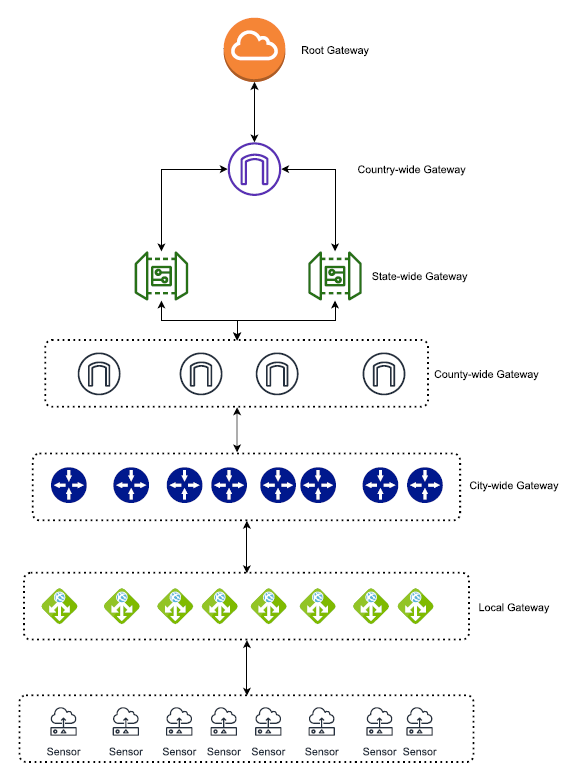
\includegraphics [width= \columnwidth]{IoTnaming.png}
 \caption{Typical hierarchical structure of the search engine \\
from \cite{main}}
 \end{figure}
Every search in the network can be specified to filter for different parameters, be they  location, availability of resources, or accuracy of sensor data. These requests can also carry their own information like urgency, user type or the time to live of the request to enable the system to prioritize searches. These search queries are handled by a Query Engine. This engine acts as an intermediary between users and devices to process queries and provides results based on the given parameters. W. G. Hatcher et al. propose that this intermediary engine has to be composed of interchangeable software components specialized for the various needs of different users. This allows for decentralized as well as specialized gateway networks depending on the local environment. The following components have been highlighted as critical:
 \subsection{Query Aggregation}
It has been theorized that many user searches will follow similar patterns and try to access overlapping resources. This in turn leads to large amounts of redundant searches. These can be aggregated by the system to significantly reduce the number of accesses needed on the individual nodes. \par
On top of the load reducing effect, query aggregation is noted to be useful for network usage analysis, making it possible to predict upcoming queries, detect attacks and make data volume assessments over time.
 \subsection{Query Prediction}
The biggest hurdle to achieve real-time IoT services has been identified as the time it needs to conduct a search, wait for the data to be generated or retrieved and then being brought back to the user in a busy network. To this end, it has been proposed to utilize a prediction algorithm to fetch time-sensitive data before they are requested by users. That makes them available in a database as soon as the query is conducted, significantly reducing network time and traffic. \par
To predict which resources will be requested in the future, patterns have to be identified and analyzed. It is assumed that these patterns are predictable for most services on a global scale within a manageable margin of error. To implement this, the use of recursive neural networks (RNNs) has been proposed. These deep learning networks are capable of incorporating their own previous predictions into their calculating, making them capable of keeping a 'memory'. They thus shall be used to make time-series forecasts of upcoming searches, as these networks are useful for self-correcting and periodically updating predictions.
 \subsection{Naming Service}
It is reasoned that existing naming services like DNS are not ideal for IoT systems. To provide a more hardware and location oriented solution, the naming system proposed in the earlier work \cite{mainPrevious} incorporates the type of device and resource, the physical location of the device based on the gateway and whether it is a publishing or subscribing node in the network. This name can be translated by the gateways into IP-addresses to allow for conventional internet communication. This is especially important in cases where users need continuous data streams from devices, which would strain the network if conducted via repeated queries for data updates. \par
 \vspace{5mm}
There are a number of theoretical implementations given in the paper that utilize these three modules. Smart transportation (being the enhancement of transportation with smart devices) is the most prominent and typical use of IoT technology according to the authors. The real-time supply of information about upcoming traffic, available parking space and environmental conditions like rain along a proposed route is introduced as a way to increase the efficiency of street transportation. By illustrating how a vehicle automatically connects to local gateways and searches for these information, the interactions between the query prediction, query aggregation and naming service are highlighted. \par
In addition to the theoretical examples, a case study on real-world data has been conducted to train a neural network for query prediction. As the data set, the available parking space over several months on 11 different parking lots in Aarhus, Denmark and Silver Springs, Maryland, USA were used to represent these queries. The performance of neural networks trained on single parking lots was compared to that of a network training on a bulk input of all lots. While a single network making these predictions for all lots would reduce the computational load significantly, it also comes with a sharp loss in accuracy. Since this case study is not representative of large-scale systems, no verdict is made on the trade-off between invested computation and accuracy achieved. \par
The paper also reviews related research and open problems. Efficiency, security and intelligence are as discussed further down the main concerns of the authors in terms of open research questions. Additionally, the deployment of the RNN is highlighted as an unsolved problem because there is little data to train it on available. To make the search engine viable, it needs to be able to provide accurate and reliable service to it's users, so any query aggregation and prediction needs to provide a certain quality from the first day on to qualify for public use.



 \section{Discussion}
%Context of current research
Research into recursive neural networks has been conducted for more than 50 years, and many uses for this kind of algorithm have been proposed. Today, the focus on RNNs lies with predicting probabilistic data, that is data that may fall in a range of possible, randomly determined values \cite{RNNrandom}. This is in line with the paper's proposed usage for a RNN, as human user queries will never be completely predictable. Hush et al. show in their paper that a pure RNN is not capable of training on truly random data without degenerating over time. They propose methods to prevent and reduce this degeneration, which may be critical in implementing a machine learning algorithm in a IoT search engine for query prediction purposes. \par
The interaction between artificial intelligence algorithms and IoT systems is becoming the topic of many research papers over the recent years. Since computer learning algorithms need large data sets to be trained on, automatic data generation is playing a increasingly larger role in research. At the same time, IoT applications can generate large amounts of data that needs to be analyzed automatically. In papers like "Count Estimation With a Low-Accuracy Machine Learning Model"  \cite{count}, new methods to combine the strengths of both systems are proposed to utilize the potential of these technologies. Here, object count systems with low inherit accuracy are being improved upon by applying Bayesian filters on classification matrices to reduce error rates. This is important for contexts where large computational power is not available, which is a common restriction of IoT devices. \par
Advances in IoT searches like \cite{webOfThings} can likely be utilized and combined with the proposed framework. Instead of looking for sensors and data sources directly, the approach allows to search for real-world entities like places or objects. Instead of asking for the value of a sensor and then computing the status of the entity, the status can be provided via an API directly. This in turn can be used to simplify the query and help aggregation, further easing the load on the network. This in turn means that the data has to be interpreted prior to being sent to the user, generating a need for processing power in the network that goes beyond sending and sorting raw data. \par
But in order to make use of these advances, the infrastructure to make IoT devices searchable needs to exist. While todays web search engines are able to access sites they are looking for to increase their accuracy, IoT search engines often don't have this capability. As highlighted in \cite{searchLessons}, the problems of searching for IoT devices lies in the fact that most devices are part of a network and don't identify themselves openly to the wider internet, often using private or manufacturer-specific identifiers. While it has been proposed in the main paper that each device gets a name that states all these things to allow for searches, these names have to be given by some overarching entity. Because of this, any IoT search engine needs to be capable of looking at the context of a device to accurately determine the services it can describe, categorising them according to it's own capabilities. \par
\cite{main} makes many assumptions about the state of tech in all these things. While there is basic work done in RNN search prediction, IoT search paradigms and device identifying algorithms, most of these are not yet developed enough to create market-ready applications. It will likely still take a lot of time to connect all the individual building blocks of such a system.



 \section{ELSI}
%What are the ethical, legal and social implications of this research?
In it's essence, the proposed research would enable individuals to access already present resources to optimize existing tasks. This could help increase efficiency of everyday processes and increase the standard of living for its users, especially in cities. \par
Assuming a widespread use, the largest recognized challenges when working with IoT technology are privacy and data security. While the supply with accurate data is beneficial to many processes, the collection of said data compromises the privacy of the user. Since this service does not exist in a vacuum and is provided by some individual or business, said provider is trusted with keeping the information safe. Following contemporary business models, it can be assumed that the service is provided in exchange for the right to analyze the data in order to sell it to a third party or use it for advertisement. While this is not a new problem, the additional capabilities of tracking an individual in real-time gives an even deeper insight and perpetuates an already unsolved concern. \par
The greater availability of IoT devices is also an already existing problem. These devices are often not sufficiently protected from tampering or illegitimate access by third parties. This is currently confined to singular networks with each security breach, as they are seldom connected to one another, making large-scale misuse infeasible. By connecting many local networks of sensors and implementing a method to access every node of all networks, every security breach has the potential to compromise the entire system. This could allow others to track and monitor individuals or even gain control about the information an individual receives. While misinformation is an already known problem, any manipulation of critical systems like for example of transportation infrastructure might prove to be directly hazardous to targeted users. This could also open up new physical security vulnerabilities, depending on connected systems. \par
Both these concerns will likely also open up new legal challenges. Most laws are not written with the capabilities of fully-connected IoT networks in mind. Problems might include copyrights, as any data a sensor generates might be considered the property of the owner, needing explicit consent to be used. Also, the unsupervised tracking of user behaviour might be unlawful in some legislatures, making a machine learning approach to query prediction impossible. \par
Lastly, any region that implements these systems might see a noticeable difference in the standard of living between users and non-users. Wherever an IoT data stream might help with a task, individuals have no equal chance of success when one side has access to this system and the other does not. An example would be the 'smart parking' example given in the paper, where individuals with a vehicle that can draw on marking lot data has a clear advantage to find a parking space over someone that doesn't. This might lead to a two-class divide in a society between individuals capable and those not capable of utilizing said system.



 \section{Outlook}
%what questions are still open? Which topics are already in active research?
Because of the inherent limitations of IoT devices in terms of computation capabilities, any overlaying system has to perform the bulk of data analysis and processing. While the proposed framework reduces network traffic and workload, the performance of the search engine still also relies on the structure of the network. While a tree hierarchy is easily scaleable from local to global scopes, it is not the most efficient network structure for large quantities of heterogeneous data packets. This may limit the systems efficiency and needs further research, as it is not touched upon in the paper. \par
A point the case study could not cover is that IoT searches do not happen in a static context where data is reliably supplied at fixed intervals. This is important as conventional neural networks have, as remarked in \cite{RNNrandom}, difficulties training and operating on inhomogeneous and unpredictable data sets, degenerating over time. The paper acknowledges the limitation in this regard, but cannot offer a solution or prediction, so that further research to implement a method to harden the RNN against these influences might be needed. \par
A system in an IoT context also has to deal with large amounts of redundancies and overlapping data sets. Machine learning can increase the performance of the system by assisting query prediction and is suspected to be able to perform query aggregation, but no large scale data processing procedure has been proposed in the paper. It may be necessary to find data mining approaches capable of processing the aggregated data. There is already research done on utilizing big data analytics on real-world statistics to make predictions about human actions, namely \cite{crime}. The team focus on identifying patterns in crime statistics, but also notes that the scope of their work is intended to be broadened in the future to also process other kinds of statistical data. \par
Lastly, for any number of devices to communicate with each other, standardized protocols and interfaces need to be agreed upon. While this framework allows for any kind of device to connect to a fitting module that ties into the local gateway, these modules still need to be developed. There is also not yet a standard protocol proposed for gateways to connect to each other outside of the naming system. Since it can be expected that large quantities of searches will be conducted automatically, these may lend themselves to more machine-near protocols to increase performance. These standards also need to keep current cybersecurity concerns and possible IoT device limitations in mind to prevent misuse of such a system. \par
This method consists of handover phrases providing secure connections and route optimizations to reduce data leakage by minimizing the relay points. This is so far only considered for distributed IP mobility management solutions, but should be able to be expanded for other systems.



% trigger a \newpage just before the given reference
% number - used to balance the columns on the last page
% adjust value as needed - may need to be readjusted if
% the document is modified later
% \IEEEtriggeratref{8}
% The "triggered" command can be changed if desired:
% \IEEEtriggercmd{ \enlargethispage{-5in}}

% references section

% can use a bibliography generated by BibTeX as a .bbl file
% BibTeX documentation can be easily obtained at:
% http://mirror.ctan.org/biblio/bibtex/contrib/doc/
% The IEEEtran BibTeX style support page is at:
% http://www.michaelshell.org/tex/ieeetran/bibtex/
% \bibliographystyle{IEEEtran}
% argument is your BibTeX string definitions and bibliography database(s)
% \bibliography{IEEEabrv,../bib/paper}
%
% <OR> manually copy in the resultant .bbl file
% set second argument of \begin to the number of references
% (used to reserve space for the reference number labels box)
% \begin{thebibliography}{1}
 \bibliography{citations}
 \bibliographystyle{unsrt}
% \bibitem{IoT:definition}
%Patel, Keyur \& Patel, Sunil \& Scholar, P \& Salazar, Carlos. (2016). \ \
%Internet of Things-IOT: Definition, Characteristics, Architecture, Enabling Technologies, %Application \& Future Challenges. 


% \end{thebibliography}



% that's all folks
 \end{document}


